% Copyright (c) 2019 FLAG lab

\documentclass[american]{flag}

\everymath{\displaystyle}

\usepackage{mathtools}
\usepackage{bm}
\usepackage{siunitx}
\sisetup{group-separator={,}, group-minimum-digits=4, per-mode=symbol, detect-all}
\usetikzlibrary{positioning, arrows.meta, fit, backgrounds, calc, shapes.geometric, decorations.pathreplacing}

\newcommand{\E}{\mathbb{E}}
\newcommand{\R}{\mathbb{R}}
\newcommand{\vtheta}{\bm{\theta}}
\newcommand{\Kset}{\mathcal{K}}
\newcommand{\Mset}{\mathcal{M}}
\newcommand{\Nset}{\mathcal{N}}
\newcommand{\argmax}{\operatorname*{arg\,max}}
\newcommand{\argmin}{\operatorname*{arg\,min}}

\newenvironment{keyidea}
  {\par\medskip\noindent\begingroup\linespread{1.25}\selectfont
   \begin{tabular}{@{}p{0.97\linewidth}@{}}\toprule\textbf{Key idea.}\ }
  {\\\bottomrule\end{tabular}\endgroup\par\medskip}

\newenvironment{wherelist}
  {\par\noindent where\begin{itemize}[nosep, leftmargin=1.6em, label=\textendash]}
  {\end{itemize}\par\smallskip}



\begin{document}

\frontmatter
\KOMAoptions{open=left}
\thispagestyle{empty}

% Copyright (c) 2019 FLAG lab

% Minimal information to be in the cover page:
% - Thesis title
% - Authors full name
% - Date of the defense (Month-yeat)
% - The text "Thesis presented for the fulfillment of the degree of DEGREE in Engineering
% - Name of the faculty
% - Name and logo of the program and research lab

\newcommand{\Author}{Juan Felipe Hernández Páez}
\newcommand{\MainTitle}{Dynamic Decentralized Aggregation for Federated Multi-Agent Reinforcement Learning in V2V Communications}
\newcommand{\SecondaryTitle}{}
\newcommand{\ShortSecondaryTitle}{Decentralized aggregation and individual reward in V2V}
\newcommand{\PublicDefenceDate}{\today}


\titlehead{%
 \begin{minipage}{0.5\textwidth}
 \centering
   \begin{flushleft}
  
\includegraphics[height=1.5cm]{figures/logo_misis}
  \end{flushleft}
  \end{minipage}
 \begin{minipage}{0.5\textwidth}
  \centering
  \begin{flushright}
  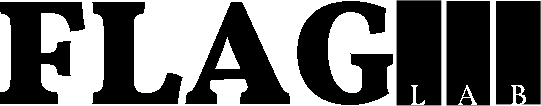
\includegraphics[height=1cm]{figures/Flag-logo}
\end{flushright}
  \end{minipage}
}

\subject{Dissertation}
\title{\MainTitle\\[.5ex]\Large\SecondaryTitle}
\author{\Author}
\date{\vskip 0.4em\normalsize{\PublicDefenceDate}}

\publishers{%
  \normalsize
  \parbox{.7\linewidth}{\centering\textsl{This thesis is submitted in partial fulfillment of the requirements \\
    for a degree of 
    Master in Systems and Computing Engineering (MISIS). %Change to specific program 
}}
  \vfill
  \begin{tabularx}{1.01\linewidth}{Xr}
    \textbf{Advisor:} & \\[1ex]
    Prof. Nicolás \textsc{Cardozo} &
     Universidad de los Andes, Colombia\\
  \end{tabularx}}

\uppertitleback{%
  {\relsize{2} \MainTitle}\\[2pt]
  {\relsize{1} \SecondaryTitle}

  \vspace{1em}%
  {\textcopyright} 2026 \Author\\[1ex]
  Systems and Computing Engineering Department\\
  FLAG lab\\ %Change to specific group
  Faculty of Engineering\\
  Universidad de los Andes\\
  Bogot\'a, Colombia
 
  \vspace{1em}%
  The experiments in this thesis were run on Hypatia, the high-performance computing cluster of
  Universidad de los Andes.

  \vspace{1em}%
  This manuscript has been set with
  \ifxetex\XeTeX\else\textsc{PDF}\LaTeX\fi\ (with
  {\textsc{Bib}\TeX} support), using the FLAG lab thesis template.  Bugs have been
  tracked down in the text and squashed thanks to \textit{Bugs in
    Writing} by \citet{dupre98bugs} and \textit{Elements of Style}
  by \citet{strunk+00style}.}

\lowertitleback{%
  \footnotesize%
  }
  
% Optional dedication page:
% \begin{flushright}
%   \dedication{DEDICATION}
% \end{flushright}

\maketitle


\endinput


% $Id:abstract.tex  $
% !TEX root = main.tex

\chapter{Abstract}



\endinput


% $Id: acknowledgements.tex 1784 2012-07-02 15:12:31Z nicolas.cardozo $
% !TEX root = main.tex

\chapter{Acknowledgements}



\endinput


\tableofcontents
\listoffigures
\KOMAoptions{open=right}

\mainmatter
%% Macros to make the title page aligned at the bottom and with a big number 
%% for the chapter number


\DeclareRobustCommand{\spacedallcaps}[1]{\textls[160]{\MakeTextUppercase{#1}}}%
\DeclareRobustCommand{\spacedlowsmallcaps}[1]{\textls[80]{\scshape\MakeTextLowercase{#1}}}%
%\newfont{\chapterNumber}{eurb10 scaled 7000}
\newfont{\chapterNumber}{pplr9d scaled 7000}
%\MakeUppercase{pplr9d scaled 7000}
\titleformat{\chapter}[display]%             
        {\relax}{\raggedleft{\color{halfgray}
        \textsc{\chaptername} \chapterNumber\thechapter}}{0pt}%
        {%\titlerule\vspace*{.9\baselineskip}
\raggedright 
\fontsize{28}{15} \selectfont           % Increase size (e.g., \LARGE, \huge, \Huge)
\bfseries%\spacedallcaps
}[\normalsize\vspace*{.3\baselineskip} \titlerule]%




\chapter{Introduction}

\section{Motivation}
% Por qué importan los enlaces V2V (avisos de seguridad con poco retardo y alta confiabilidad), cómo reutilizan los canales de la red celular y por qué elegir canal y potencia es un problema difícil que se ha abordado con MARL federado Li et al

\section{Problem statement}
% El esquema de Li et al. decide de forma descentralizada pero aprende a través de la BS (FedAvg y recompensa compartida). Preguntas de investigación: PI1, quitar la BS de la agregación de modelos; PI2, usar una recompensa individual por agente.

\section{Objectives}
% Objetivo general (diseñar, implementar y evaluar la arquitectura descentralizada con recompensa individual) y lista de objetivos específicos.

\section{Contributions}
% Las tres contribuciones: implementación verificada y reproducible del esquema de Li et al., agregación descentralizada por gossip entre vecinos y recompensa individual por agente.

\section{Scope}
% Límites del trabajo: todo es simulación, una sola celda con 15 CUE y 5 a 30 pares V2V, simplificaciones frente al artículo original y posiciones fijas dentro de cada episodio.

\section{How to read this document}
% Para quién está escrito el documento, qué capítulo explica los conceptos desde cero y qué ayudas de lectura tiene (resúmenes de ideas clave, explicación de los símbolos después de cada ecuación).

\section{Document structure}
% Un párrafo que resume qué contiene cada capítulo y cada apéndice.

\chapter{Background}

\section{Vehicular communications and spectrum reuse}
% Lo necesario de comunicaciones inalámbricas para entender el modelo: interferencia, calidad de una señal y relación entre cola y retardo.

\subsection{Vehicle-to-vehicle links and the cellular network}
% Qué son V2X y V2V, qué es un par V2V, qué mensajes lleva y cómo reutiliza los canales de subida de los CUE a costa de interferirlos.

\subsection{Power and decibels}
% Escala logarítmica: razones de potencia en dB y potencias absolutas en dBm, con ejemplos de conversión.

\subsection{Channel gain: distance and fading}
% La ganancia h = alpha * g: pérdida por distancia (gran escala) y desvanecimiento rápido (pequeña escala).

\subsection{Signal-to-interference-plus-noise ratio}
% Definición de la SINR, potencia del ruido térmico e interferencia de otros transmisores en el mismo canal.

\subsection{Channel capacity}
% Fórmula de Shannon, R = W log2(1 + SINR), y cómo crece la tasa con la SINR.

\subsection{Queues, delay, and Little's law}
% Cómo crece y se vacía una cola según la tasa de llegada y la de transmisión, y la ley de Little, que relaciona el tamaño de la cola con el retardo.

\section{Reinforcement learning}
% Cómo aprende un agente por refuerzo, desde la interacción con el entorno hasta Q-learning.

\subsection{Agent, environment, and reward}
% El ciclo estado, acción, recompensa y nuevo estado, y qué es una política.

\subsection{Return and discount factor}
% El retorno como suma descontada de recompensas y el papel del factor de descuento gamma.

\subsection{Markov decision processes}
% Los cinco elementos de un MDP y la propiedad de Markov.

\subsection{Value functions and the Bellman equation}
% La función Q de una política, la función Q óptima y la ecuación de Bellman.

\subsection{Q-learning}
% La regla de actualización de Q-learning y el error de diferencia temporal (TD).

\subsection{Exploration versus exploitation}
% La política epsilon-greedy y cómo se reduce epsilon durante el entrenamiento.

\section{Deep reinforcement learning}
% Cómo se combina el aprendizaje por refuerzo con redes neuronales y las mejoras que forman el agente D3QN.

\subsection{Neural networks as function approximators}
% Por qué no sirve una tabla cuando el estado es continuo y cómo una red neuronal con pesos theta aproxima la función Q.

\subsection{Deep Q-networks}
% La pérdida de la DQN, el buffer de repetición de experiencia y la red objetivo Mnih et al.

\subsection{Double DQN}
% Por qué el máximo sobrestima los valores y cómo la doble DQN separa elegir la acción de evaluarla.

\subsection{Dueling architecture}
% Estimar por separado el valor del estado V(s) y la ventaja A(s, a), y cómo se combinan en Q.

\subsection{Prioritized experience replay}
% Muestrear las transiciones según su error TD, el exponente de prioridad y los pesos de importancia que corrigen el sesgo.

\subsection{Huber loss}
% Pérdida cuadrática para errores pequeños y lineal para errores grandes, para evitar saltos bruscos en los pesos.

\subsection{The D3QN network}
% Cómo se combinan duelo, doble DQN y PER en el agente que usa cada par V2V.

\section{Multi-agent reinforcement learning}
% Qué cambia cuando aprenden varios agentes a la vez en el mismo entorno.

\subsection{From one agent to many}
% Agentes que comparten un entorno, la acción conjunta y la formalización como Dec-POMDP.

\subsection{Why it is hard}
% Las cuatro dificultades propias del caso multiagente: observabilidad parcial, no estacionariedad, escalabilidad y asignación de crédito.

\subsection{Ways to train multiple agents}
% Entrenamiento y ejecución centralizados, CTDE y DTE (clasificación de Amato), y dónde encaja el aprendizaje federado.

\section{Federated learning}
% La idea del aprendizaje federado y su aplicación al aprendizaje por refuerzo.

\subsection{The idea and the FedAvg algorithm}
% Entrenar sin mover los datos: copias locales del modelo, un servidor que promedia y la fórmula de FedAvg (McMahan et al).

\subsection{Federated reinforcement learning}
% Aplicar el promedio federado a agentes de refuerzo; FRL horizontal, que es el caso que uso.

\subsection{The cost of the central server}
% El servidor como punto único de falla, cuello de botella de la comunicación y entidad en la que todos deben confiar.

\section{Decentralized federated learning and gossip}
% Cómo aprender sin servidor, intercambiando modelos solo entre vecinos.

\subsection{Communication graph}
% Nodos, aristas, vecinos y grado; grafos geométricos aleatorios como modelo de una red inalámbrica.

\subsection{Averaging with neighbors}
% Algoritmos de gossip: una ronda de promedio con los vecinos y cómo la estructura del grafo determina la velocidad de convergencia al consenso.

\subsection{Learning and averaging at the same time}
% Combinar pasos de entrenamiento local con rondas de promedio (D-PSGD de Lian et al) y su costo de comunicación frente a la versión centralizada.

\chapter{Related work}

\section{Reinforcement learning for V2V resource allocation}

\section{Federated and multi-agent reinforcement learning}

\section{Serverless decentralized learning}

\section{Reward design in multi-agent systems}

\section{Positioning of this thesis}

\chapter{System model and problem formulation}

\section{Scenario}
% Celda de 500 m de radio con la BS en el centro, 15 CUE con un canal de subida cada uno, K pares V2V (5 a 30), cómo se sortean las posiciones y quiénes son vecinos (300 m o menos).

\section{Channel model}
% Las ganancias de todos los enlaces (gran y pequeña escala), la distancia mínima y qué ganancias conoce cada agente.

\section{Signal quality and rates}
% SINR de cada CUE en la BS y de cada par V2V, y las tasas de Shannon que resultan.

\section{Queue and delay}
% Dinámica de la cola de cada transmisor con llegada constante de 1 Mbps, el desborde y la relación con el retardo.

\section{Reliability}
% Probabilidad de interrupción (outage) con umbral de 5 dB y p_o = 0.1, y cómo se convierte en un umbral sobre la ganancia del enlace.

\section{The optimization problem}
% Maximizar la suma de las tasas de los CUE sujeta a tasa mínima, retardo máximo y confiabilidad de los pares, como lo plantean Li et al

\section{Formulation as a multi-agent learning problem}
% Cada par V2V es un agente; juntos forman un Dec-POMDP.

\subsection{Observation}
% El vector de 46 números que observa cada agente: su enlace en cada canal, cada CUE hacia la BS, vecinos en cada canal y su cola.

\subsection{Action}
% La pareja canal y potencia: 15 canales por 4 niveles, 60 acciones.

\subsection{Shared reward}
% La recompensa compartida que calcula la BS al final de cada slot: términos de tasa de los CUE, de colas y de confiabilidad de los pares, con sus pesos lambda.

\subsection{Objective of each agent}
% Cada agente maximiza su retorno descontado; con la recompensa compartida debe descubrir qué parte del resultado depende de su propia acción.

\subsection{What happens in a slot}
% El orden de los eventos en un slot: observar, elegir, calcular SINR, tasas y colas, recibir la recompensa y aprender.

\chapter{Proposed architecture}

\section{The agent of each pair}

\section{Centralized aggregation: FedAvg}

\section{Decentralized aggregation by gossip}

\subsection{Why averaging with neighbors makes sense}

\subsection{Variant with at most \texorpdfstring{$S$}{S} neighbors}

\section{Individual reward}

\section{Resulting methods}

\section{Communication cost}

\chapter{Implementation}

\section{Code organization}
% Las tres partes del código (entorno, agentes y programas de entrenamiento y análisis), la tabla de módulos y por qué la separación sigue a la del modelo.

\section{The environment}
% El entorno con la interfaz paralela de PettingZoo: reset y step, el sorteo de posiciones con la semilla y el cálculo de SINR, colas y recompensas.

\section{The agents and the aggregation}
% Cada agente como objeto con sus redes, su buffer, su optimizador y su generador aleatorio, y la implementación de FedAvg y gossip (con un fragmento de código).

\section{Verification}
% Las 191 pruebas automáticas y sus tres tipos: fórmulas comparadas con valores calculados a mano, propiedades e integración.

\section{Running on the cluster}
% La ejecución en Hypatia con Slurm: recursos por corrida, cómo se agrupan las semillas en trabajos y cómo se describe cada barrido.

\section{From the logs to this document}
% Cómo las tablas y figuras de resultados se generan automáticamente a partir de los registros de las corridas.

\section{Differences from the original paper}
% Tablas con cada diferencia frente a Li et al. (simplificaciones del canal, la geometría y el tráfico, y valores que el artículo no reporta) y su justificación.
 % posible eliminar
\chapter{Experimental setup}

\section{Parameters}
% Tablas de parámetros del escenario, el canal y la recompensa, y de los agentes y la agregación, indicando de dónde sale cada valor.

\section{Compared methods}
% Las dos reglas fijas (Greedy y la regla de umbral) y los tres métodos que aprenden (DTE, FedAvg y gossip).

\section{Runs}
% Qué es una corrida (un método, un K y una semilla durante 2000 episodios) y los cuatro barridos: recompensa individual, recompensa compartida y gossip con S = 2 y con S = 3.

\section{Metrics}
% Recompensa por episodio (medida principal), valor final y medidas de calidad de servicio, comportamiento, comunicación, consenso y aprendizaje.

\section{How the methods are compared}
% Comparaciones pareadas semilla por semilla, prueba de signos y lo que no se compara.

\chapter{Results}

\section{Does the implementation reproduce the original scheme?}

\section{Diagnosis: why the original scheme degrades}

\section{Individual reward versus shared reward}

\section{Gossip aggregation versus FedAvg}

\section{The complete proposal versus the original scheme}

\section{Learning speed and stability}

\section{What the agents learn}

\section{Neighborhoods and consensus}

\section{Communication cost}

\section{The threshold rule as a reference}

\section{Discussion}

\section{Threats to validity}

\chapter{Conclusions}

\section{Answers to the research questions}
% Respuesta directa a PI1 (quitar la BS de la agregación) y a PI2 (recompensa individual), con los números principales.

\section{Contributions}
% Las tres contribuciones y lo que se logró con cada una.

\section{Other findings}
% Hallazgos secundarios: el factor de descuento importa, compartir con todos no siempre ayuda, FedAvg aprende rápido pero olvida y una regla simple sigue siendo mejor.

\section{Limitations}
% Simulación simplificada, recompensa individual que no es del todo local, intercambios ideales y demasiado frecuentes, evidencia estadística moderada y distancia a lo que es posible lograr.

\section{Future work}
% Escenarios más realistas, mejores recompensas, comunicación más barata y realista, entender por qué ayudan los vecinos, acercarse a la regla de umbral y robustez.



%Adding appendices if needed
\appendix
\chapter{Notation}
% Tabla de los símbolos del documento agrupados por tema, con la ecuación o sección en que se definen, y aclaración de las letras con dos usos.

\chapter{Detailed results}

\section{Variability across seeds}

\section{Computation time}

\chapter{Reproducibility}

\section{Software}

\section{Repository organization}

\section{Steps}

\section{Seeds}


\backmatter
\bibliography{bib/local,bib/writing}

\printindex
\addcontentsline{toc}{chapter}{List of Terms}
\printindex[symbols]
%----[ Acronyms ]---

\chapter*{Acronyms}

\addcontentsline{toc}{chapter}{Acronyms}
\begin{acronym}[Dec-POMDP]

%\acro{ACRONYM}{LONG_NAME}
\acro{BS}{base station}
\acro{CRDT}{conflict-free replicated data type}
\acro{CTDE}{centralized training with decentralized execution}
\acro{CUE}{cellular user}
\acro{D3QN}{dueling double deep Q-network}
\acro{Dec-POMDP}{decentralized partially observable Markov decision process}
\acro{DFL}{decentralized federated learning}
\acro{DQN}{deep Q-network}
\acro{DTE}{decentralized training and execution}
\acro{FedAvg}{Federated Averaging}
\acro{FL}{federated learning}
\acro{MARL}{multi-agent reinforcement learning}
\acro{MDP}{Markov decision process}
\acro{PER}{prioritized experience replay}
\acro{RL}{reinforcement learning}
\acro{SINR}{signal-to-interference-plus-noise ratio}
\acro{V2V}{vehicle-to-vehicle}

\end{acronym}

%\newcommand{\acResetNonTrivial}
%  {\acresetall
%   \acused{CPU}
%   \acused{API}}

%\acResetNonTrivial


\end{document}

\endinput

